%% AQB conference version. ACM sigconf, camera-ready, named authors.
%% Build: latexmk -pdf main.tex   (figures: python3 make_figs.py; numbers: ../data/*.json)
\documentclass[sigconf]{acmart}

\usepackage{booktabs}
\usepackage{multirow}
\usepackage{tikz}
\usetikzlibrary{positioning,arrows.meta,shapes.geometric,fit,calc}
\usepackage{xspace}
\usepackage{enumitem}
\usepackage{listings}
\lstset{basicstyle=\ttfamily\scriptsize, breaklines=true, columns=fullflexible, frame=single,
  framerule=0.3pt, xleftmargin=2pt, xrightmargin=2pt}

\newcommand{\aqb}{AQB\xspace}
\newcommand{\rqref}[1]{\textbf{RQ#1}}
\newcommand{\answer}[2]{\smallskip\noindent\textit{Answer to RQ#1.} #2\smallskip}

\setcopyright{none}
\settopmatter{printacmref=false}
\renewcommand\footnotetextcopyrightpermission[1]{}


\begin{document}

\title[Can LLM Agents Hold the Release Gate?]{Can LLM Agents Hold the Release Gate?\\
A Benchmark of Device-Verified Regressions in Real Android Apps}

\author{Mayank Singh}

\begin{abstract}
Coding agents now produce code changes faster than people can test them, so the release gate, a
human tester who exercises what changed and either files bugs or signs off, is becoming the
bottleneck. We ask whether a large language model (LLM) agent can hold that gate, and whether its
reports and sign-offs can be trusted. We present \aqb, a benchmark of 51 release-QA episodes over
9 open-source Android apps. Each episode is a build with one to three planted regressions, 92 in
total (91 observable). Each regression is a real upstream bug, re-introduced on a pinned head commit
and verified on a device by target, held-out and preservation checks. The agent receives release
notes that name every changed feature without stating a symptom, drives an Android~15 device only
through screen tools, files structured bug reports, and decides when to sign off. A deterministic
matcher grades the reports without a model judge. Across six agent configurations from three
providers, the best recall is 59.3\% and the best strict pass rate (every regression reported, then a
sign-off) is 29.4\%; 17 of the 91 observable regressions escape every configuration. Agents reach
74--96\% of the changed features but rarely run the checks that expose the regressions: re-opening
after a change, specific inputs, and comparing a value with what it should be. The confidence an
agent states with its sign-off is close to chance at telling a correct sign-off from an incorrect one
(area under the ROC curve 0.33--0.58). The highest-recall and the highest-scoring configurations
differ, but neither difference survives correction for multiple comparisons. We report the grader's
validation and failure modes and the confounds we found in the runs.
\end{abstract}

\begin{CCSXML}
<ccs2012>
<concept><concept_id>10011007.10011074.10011099.10011102.10011103</concept_id>
<concept_desc>Software and its engineering~Software testing and debugging</concept_desc>
<concept_significance>500</concept_significance></concept>
<concept><concept_id>10010147.10010178</concept_id>
<concept_desc>Computing methodologies~Artificial intelligence</concept_desc>
<concept_significance>300</concept_significance></concept>
</ccs2012>
\end{CCSXML}
\ccsdesc[500]{Software and its engineering~Software testing and debugging}
\ccsdesc[300]{Computing methodologies~Artificial intelligence}

\keywords{LLM agents, release testing, regression testing, test oracle, Android, GUI testing, benchmark}

\maketitle
\pagestyle{plain}

%% ------------------------------------------------------------------------------------------
\section{Introduction}

A team that uses coding agents can produce changes faster than people can test them. In many teams
the last check before release is still a tester who reads the release notes, exercises what changed,
and either files bugs or signs off. That person acts as the \emph{test oracle}: the judge of whether
observed behaviour is correct. When no specification or automated oracle is adequate, the human
remains the final source of oracle information~\cite{barr2015oracle}. The task combines
\emph{regression testing}, which gives confidence that changes do not harm existing
behaviour~\cite{yoo2012regression}, with \emph{exploratory testing}, in which learning, test design
and test execution happen together~\cite{itkonen2005exploratory}.

Two questions decide whether an LLM agent can take this role: does it catch the regressions that are
actually there, and can its reports and sign-offs be trusted? Current benchmarks measure other
things. Software-engineering agent benchmarks grade code that an agent
writes~\cite{jimenez2024swebench,merrill2026terminalbench}. Computer-use and Android agent benchmarks
grade whether an agent completes a task in an app assumed to be
correct~\cite{rawles2025androidworld,xu2025androidlab,xie2024osworld}. Android testing research
measures test generators on coverage and crashes~\cite{li2017droidbot,mao2016sapienz,su2017stoat,su2021themis},
and recent tools target non-crashing functional bugs with automatic or model-based
oracles~\cite{su2021genie,wang2022deepstate,liu2025visiondroid,liu2025guipilot}. To our knowledge,
no benchmark asks an LLM agent to act as a release gate: to sweep a build from its release notes,
report the regressions it finds, and decide when the build may ship.

\aqb is built for this question (Figure~\ref{fig:overview}). Each of its 51 episodes is a pre-release
sweep of one build that contains one to three planted regressions. The agent receives a short brief,
the seeded data, and a \emph{Changed in this build} list written like real release notes. The list
names every changed feature without a symptom or trigger, and mixes in harmless changes. The agent
tests the app on a device through screen tools, files bug reports to a scripted developer, and signs
off when it judges the build ready.

This paper makes four contributions:
\begin{itemize}[leftmargin=*]
\item a benchmark of 92 planted, device-verified regressions (91 observable) in 9 real Android apps,
  organised into 51 release-QA episodes with 92 real and 93 decoy release-note lines
  (Section~\ref{sec:benchmark});
\item a deterministic, model-free matcher for free-text bug reports, anchored to what was on screen,
  validated on 1,212 reports, with its failure modes measured (Section~\ref{sec:grading});
\item an evaluation of six agent configurations from three providers, each in its vendor's own
  harness, with intervals, pairwise tests corrected for multiple comparisons, and sensitivity analyses
  (Sections~\ref{sec:setup} and~\ref{sec:results});
\item a per-feature account of every miss (never reached, reached but not exercised, or exercised but
  not noticed), a description of the regressions that the two leading configurations both miss, and a
  list of the confounds in the runs (Sections~\ref{sec:rq4} and~\ref{sec:threats}).
\end{itemize}

\begin{figure*}[t]
  \centering
  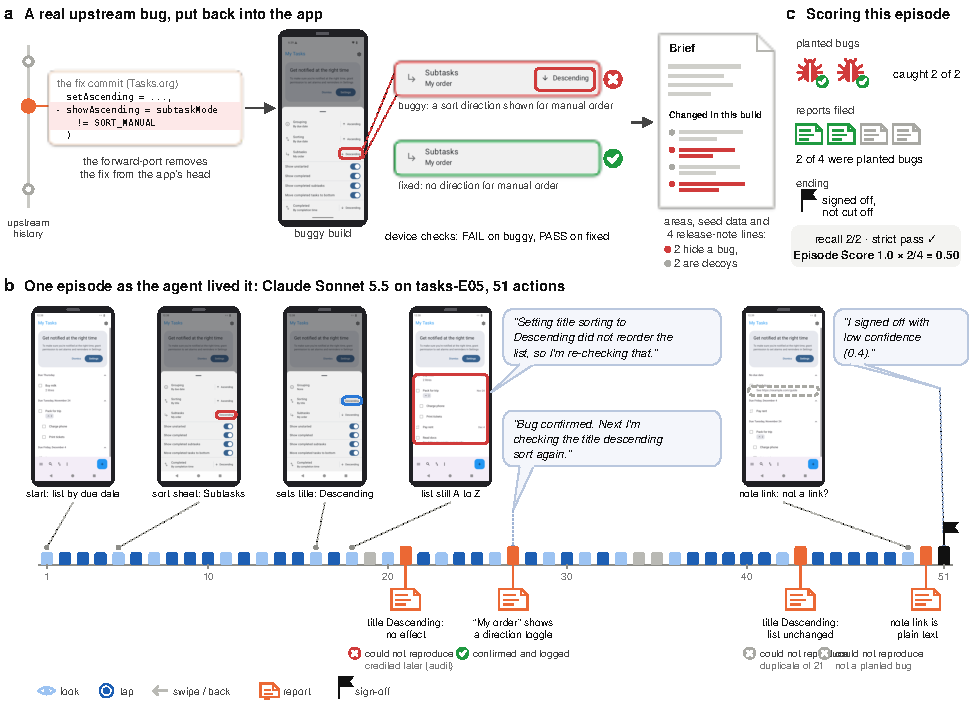
\includegraphics[width=\textwidth]{../figures/p0_overview.pdf}
  \caption{\aqb at a glance, with real artifacts from one episode. \textbf{a}, A regression enters a
  build: the fix commit of an upstream bug in Tasks.org is reversed on the app's pinned head. On a
  device the buggy build shows a sort-direction toggle for a manually ordered list, which the fixed
  build does not show; the bug's checks fail on the buggy build and pass on the fixed one. The brief
  lists four changed features, two of which hide regressions (colours are for the reader; the agent
  sees plain lines). \textbf{b}, The same episode as executed by Claude Sonnet~5.5: its screenshots,
  its own words, each of its 51 actions by type, the four reports it filed with the scripted
  developer's replies, and the sign-off. \textbf{c}, How this episode is scored.}
  \Description{Three-panel overview: how a regression is planted, a timeline of one agent's 51
  actions with its reports, and the scoring of that episode.}
  \label{fig:overview}
\end{figure*}

In short, no configuration we evaluated is a reliable release gate. The best recall is 59.3\% and
the best strict pass rate is 29.4\%. Agents reach most changed features but rarely run the specific
check that exposes the regression, most sign-offs leave regressions in the build, and the stated
confidence does not indicate whether a sign-off is correct. Catches overlap more than chance across
configurations.

%% ------------------------------------------------------------------------------------------
\section{Background and Related Work}
\label{sec:related}

\paragraph{The test oracle problem.}
Deciding whether an observed behaviour is correct is the oracle problem. Its automated solutions
include specifications, models, contracts and metamorphic relations, and the human remains the
fallback~\cite{barr2015oracle}. \aqb evaluates LLM agents as that fallback oracle on functional
regressions that do not crash.

\paragraph{Agent benchmarks for software.}
SWE-bench grades patches for real GitHub issues by running the repository's
tests~\cite{jimenez2024swebench}. SWE-bench Verified is a human-validated
subset~\cite{openai2024sweverified}, and Terminal-Bench grades command-line
tasks~\cite{merrill2026terminalbench}. Data leakage and weak tests can inflate such
scores~\cite{aleithan2024swebenchplus}, which motivates benchmarks built from recent
issues~\cite{zhang2025swebenchlive}. In these benchmarks the agent writes code and tests written by
people are the oracle. In \aqb the agent is the tester.

\paragraph{Mobile and computer-use agents.}
AndroidWorld~\cite{rawles2025androidworld}, AndroidLab~\cite{xu2025androidlab} and
OSWorld~\cite{xie2024osworld} measure task completion with programmatic success checks in apps that
are assumed to be correct. OSWorld also reports a human baseline~\cite{xie2024osworld}. In \aqb the
app contains defects that the agent must discover, and success depends on the agent's judgement of
whether what it sees is correct.

\paragraph{Automated Android GUI testing.}
Random, search-based and model-based test generators such as DroidBot~\cite{li2017droidbot},
Sapienz~\cite{mao2016sapienz} and Stoat~\cite{su2017stoat} are evaluated mostly on coverage and
crashes. Themis benchmarks such tools on real crash bugs~\cite{su2021themis}. Several approaches
target non-crashing functional bugs: Genie derives oracles from an independent-view
property~\cite{su2021genie}, deep-state differential analysis flags deviant behaviour as a generic
oracle~\cite{wang2022deepstate}, and GUIPilot checks implementations against design
mock-ups~\cite{liu2025guipilot}. An empirical study of 399 functional bugs describes their symptoms
and oracles~\cite{xiong2023functionalbugs}. LLM-based testers include
GPTDroid~\cite{liu2024gptdroid}, DroidAgent~\cite{yoon2024droidagent}, QTypist for text
inputs~\cite{liu2023qtypist}, GraphDroid~\cite{li2026graphdroid}, and VisionDroid, a multimodal
tester evaluated on 590 non-crash bugs~\cite{liu2025visiondroid}. These works propose testing tools.
\aqb measures the release-gate decision itself, with release notes as the only guide and a sign-off
that ends the session. Table~\ref{tab:related} summarises the differences.

\begin{table}[t]
  \caption{\aqb compared with related benchmarks.}
  \label{tab:related}
  \footnotesize\setlength{\tabcolsep}{2.5pt}
  \begin{tabular}{@{}llll@{}}
    \toprule
    Benchmark & Agent's task & App or code & Oracle \\
    \midrule
    SWE-bench~\cite{jimenez2024swebench} & write a patch & has a known issue & repository tests \\
    Terminal-Bench~\cite{merrill2026terminalbench} & shell task & -- & per-task tests \\
    AndroidWorld~\cite{rawles2025androidworld} & Android app task & assumed correct & state checks \\
    OSWorld~\cite{xie2024osworld} & desktop task & assumed correct & execution scripts \\
    Themis~\cite{su2021themis} & generate tests & real crash bugs & crash detection \\
    \aqb (ours) & test and sign off & planted regressions & device checks, \\
     & & (non-crashing) & report matcher \\
    \bottomrule
  \end{tabular}
\end{table}

\paragraph{Real faults.}
Like Defects4J~\cite{just2014defects4j}, \aqb builds each bug from a real upstream fix. Real faults
are the reference against which mutants are validated~\cite{just2014mutants}. Unlike Defects4J, the
bug is observed only through the app's screen, and the oracle is a set of device checks rather than
a test suite.

%% ------------------------------------------------------------------------------------------
\section{The AQB Benchmark}
\label{sec:benchmark}

\subsection{Apps}
\aqb uses 9 open-source Android apps (Table~\ref{tab:apps}). Four are mature projects with long
histories. Five are projects whose entire history is from 2026. NerdCalci (a notepad calculator) and
Idle Fantasy (an idle role-playing game) are not form-and-list apps: most of their bugs are
plausible-looking wrong values that a tester must compute to catch. Each app is pinned to one head
commit.

\begin{table}[t]
  \caption{Apps and the regressions planted in their episodes. Planted counts include one
  regression (Amaze) that another bug in its episode masks; 91 are observable.}
  \label{tab:apps}
  \footnotesize\setlength{\tabcolsep}{3.5pt}
  \begin{tabular}{@{}llllrr@{}}
    \toprule
    App & Domain & Licence & History & Ep. & Regr. \\
    \midrule
    Amaze File Manager & file manager & GPL-3.0 & mature & 6 & 12 (11) \\
    AnkiDroid & flashcards & GPL-3.0 & mature & 8 & 15 \\
    Markor & Markdown editor & Apache-2.0 & mature & 6 & 13 \\
    Tasks.org & to-do lists & GPL-3.0 & mature & 6 & 12 \\
    Minus & expense tracker & Apache-2.0 & 2026 & 6 & 8 \\
    Iris Gallery & photo gallery & Apache-2.0 & 2026 & 3 & 3 \\
    Featherline & medication tracker & GPL-3.0 & 2026 & 6 & 9 \\
    NerdCalci & notepad calculator & GPL-3.0 & 2026 & 4 & 8 \\
    Idle Fantasy & idle RPG & GPL-3.0 & 2026 & 6 & 12 \\
    \midrule
    Total & & & & 51 & 92 (91) \\
    \bottomrule
  \end{tabular}
\end{table}

\subsection{Regressions}
\label{sec:regressions}

\paragraph{Mining.}
Each regression starts from a merged upstream fix that corrects behaviour a user can see. A fix is
kept when its bug (i) shows on the screen or in data the app displays, (ii) is deterministic, and
(iii) can be judged wrong by a tester without the code. Figure~\ref{fig:funnel} gives the counts. At
least 256 fixes were examined. 93 were rejected when the candidate shortlists were drawn up; these
rejections were recorded only for the later mining rounds, so the true number examined is higher. 62
were dropped after authoring and 101 were verified on a device. The most common reasons to drop a bug
were a dependency on home-screen widgets, notifications or alarms (7), pixel-level layout symptoms
(6), intents to other apps (4), and wall-clock, camera, operating-system or gesture-physics
dependencies (3 each). Of the 101 verified bugs, 92 are planted in episodes; the other 9 are used only
in single-check cases, which this paper does not evaluate. Each regression is labelled with a family:
state (38), display (35) or interaction (19).

\begin{figure}[t]
  \centering
  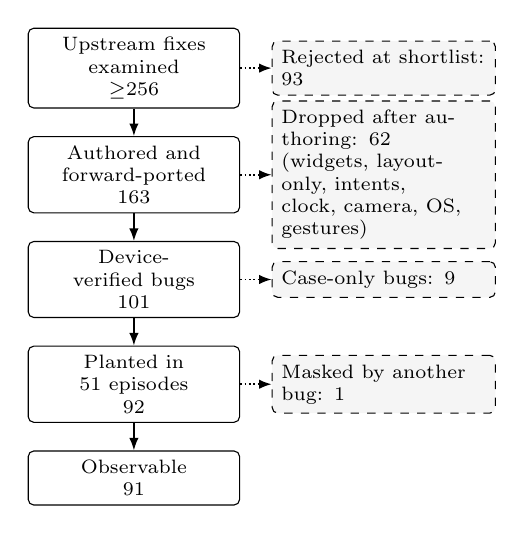
\begin{tikzpicture}[
      box/.style={draw, rounded corners=2pt, align=center, font=\scriptsize, minimum height=6mm,
                  text width=2.45cm, fill=white},
      drop/.style={draw, dashed, rounded corners=2pt, align=left, font=\scriptsize, text width=2.6cm,
                   fill=black!4},
      arr/.style={-{Latex[length=1.6mm]}, semithick}]
    \node[box] (m) {Upstream fixes examined\\$\geq$256};
    \node[box, below=3.5mm of m] (a) {Authored and\\forward-ported\\163};
    \node[box, below=3.5mm of a] (v) {Device-verified bugs\\101};
    \node[box, below=3.5mm of v] (p) {Planted in 51 episodes\\92};
    \node[box, below=3.5mm of p] (o) {Observable\\91};
    \node[drop, right=4mm of m] (d1) {Rejected at shortlist: 93};
    \node[drop, right=4mm of a] (d2) {Dropped after authoring: 62\\(widgets, layout-only, intents,\\clock, camera, OS, gestures)};
    \node[drop, right=4mm of v] (d3) {Case-only bugs: 9};
    \node[drop, right=4mm of p] (d4) {Masked by another bug: 1};
    \foreach \x/\y in {m/a, a/v, v/p, p/o} \draw[arr] (\x) -- (\y);
    \foreach \x/\y in {m/d1, a/d2, v/d3, p/d4} \draw[arr, densely dotted] (\x) -- (\y);
  \end{tikzpicture}
  \caption{Construction of the regression set. Every verified bug has target, held-out and
  preservation checks that hold on a device (Section~\ref{sec:regressions}).}
  \Description{A vertical funnel from at least 256 upstream fixes to 91 observable regressions, with
  the number removed at each stage shown on the right.}
  \label{fig:funnel}
\end{figure}

\paragraph{Forward-porting.}
Each bug is re-introduced on its app's single pinned head commit, so every bug of an app lives in one
source tree and every brief matches the current user interface. The buggy build is the head plus a
patch that reverses the fix (Figure~\ref{fig:overview}a); the fixed build is the clean head. Each port
records its approach and a confidence label (57\% high, 39\% medium, 4\% low), and every APK is
recorded with its source commit, applied patches, toolchain and SHA-256 hash.

\paragraph{Device checks.}
Each bug has three deterministic checks that seed the app, drive the device along a fixed path, and
read the screen or the app's stored data. The \emph{target} check exercises the bug's own trigger, the
\emph{held-out} check reaches the same defect by another path, and the \emph{preservation} check tests
neighbouring behaviour. A bug is accepted only if, on a device, the target and held-out checks fail on
the buggy build and pass on the fixed build, and the preservation check passes on both. Checks that
need app-private data read it through an instrumentation probe signed with the app's debug key, so no
device needs root.

\subsection{Episodes and Release Notes}
An episode groups one to three regressions of the same app whose patches touch different files (16
episodes have one regression, 29 have two, and 6 have three). Groups whose bugs interfered on the
device were split. In one pair, one bug removes the code path of the other, and that pair is scored
with the masked bug excluded. Every start build was checked on a device: each observable regression's
target check fails, and every preservation check passes.

The agent's brief names the areas to sweep, the seeded data, and a \emph{Changed in this build} list
with one line per planted regression and one or two lines for harmless changes (92 real and 93 decoy
lines in total, in mixed order). Lines are written at the level of a real changelog: they name the
feature and what changed in its mechanism (``Subtasks section of the sort sheet: its controls are now
built the same way for every option''). They never state a symptom, a trigger or an expected value,
and real and decoy lines use the same verbs. A leak scan checks that no brief contains a bug
identifier, commit wording or a code identifier from the original fix.

\subsection{Environment and Protocol}

\begin{figure*}[t]
  \centering
  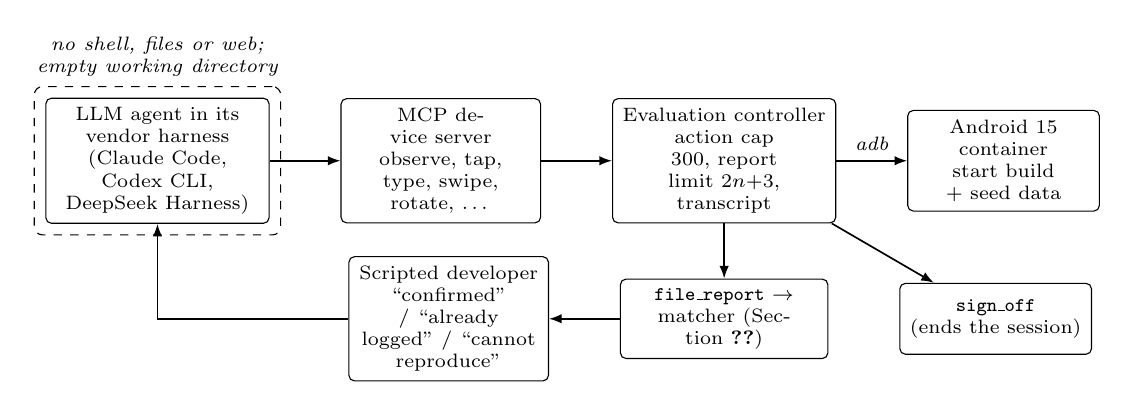
\begin{tikzpicture}[
      blk/.style={draw, rounded corners=2pt, align=center, font=\scriptsize, minimum height=9mm, fill=white},
      grp/.style={draw, dashed, rounded corners=3pt, inner sep=4pt},
      arr/.style={-{Latex[length=1.6mm]}, semithick},
      lab/.style={font=\scriptsize\itshape, align=center}]
    \node[blk, text width=2.6cm] (agent) {LLM agent in its vendor harness\\(Claude Code, Codex CLI,\\DeepSeek Harness)};
    \node[blk, text width=2.3cm, right=9mm of agent] (mcp) {MCP device server\\observe, tap, type, swipe,\\rotate, \ldots};
    \node[blk, text width=2.6cm, right=9mm of mcp] (ctrl) {Evaluation controller\\action cap 300, report\\limit $2n{+}3$, transcript};
    \node[blk, text width=2.2cm, right=9mm of ctrl] (dev) {Android 15 container\\start build + seed data};
    \node[blk, text width=2.4cm, below=7mm of ctrl] (rep) {\texttt{file\_report} $\rightarrow$\\matcher (Section~\ref{sec:grading})};
    \node[blk, text width=2.3cm, left=9mm of rep] (dvp) {Scripted developer\\``confirmed'' / ``already\\logged'' / ``cannot reproduce''};
    \node[blk, text width=2.2cm, right=9mm of rep] (so) {\texttt{sign\_off}\\(ends the session)};
    \node[grp, fit=(agent), label={[lab]above:no shell, files or web;\\empty working directory}] {};
    \draw[arr] (agent) -- (mcp);
    \draw[arr] (mcp) -- (ctrl);
    \draw[arr] (ctrl) -- node[lab, above]{adb} (dev);
    \draw[arr] (ctrl) -- (rep);
    \draw[arr] (rep) -- (dvp);
    \draw[arr] (ctrl) -- (so);
    \draw[arr] (dvp.west) -| (agent.south);
  \end{tikzpicture}
  \caption{Episode environment. The agent reaches the device only through the MCP device server;
  every call is executed and logged by the evaluation controller. Reports are graded online and
  answered by a scripted developer; under the fast protocol a confirmed regression stays in the build.}
  \Description{Block diagram: agent harness to MCP server to evaluation controller to Android
  container; reports go to the matcher and a scripted developer whose reply returns to the agent.}
  \label{fig:arch}
\end{figure*}

\paragraph{Device.}
Each episode runs on a fresh Android~15 (x86\_64) container with a $1080\times2400$ display at 420
dpi. Before the episode the device is reset, the start build is installed, the seed data is written,
and the app is opened.

\paragraph{Tools.}
The agent operates the device only through a Model Context Protocol server~\cite{anthropic2024mcp}
(Figure~\ref{fig:arch}). \texttt{observe} returns the numbered UI elements of the current screen with
their text, content descriptions, states and centres, and optionally a screenshot. \texttt{tap},
\texttt{long\_press}, \texttt{type\_text}, \texttt{swipe}, \texttt{press\_key}, \texttt{rotate},
\texttt{open\_app} and \texttt{wait} act on the device. \texttt{file\_report} and \texttt{sign\_off}
are handled by the evaluation controller. The agent harness has every other tool disabled and runs in
an empty temporary directory, so the agent cannot read the app's code, the dataset or the original
fix. A message that names an answer path disqualifies the run.

\paragraph{Prompt.}
The prompt has three parts: (i) the brief; (ii) a short, generic QA method (Appendix~\ref{app:prompt})
that asks the agent to plan every area, check state after leaving and returning, reverse and repeat
actions, try empty and boundary inputs, check consistency between screens, rotate the device and
reach screens by more than one route; and (iii) instructions for finishing.

\paragraph{Reports, developer and termination.}
A report has a screen, an element, an optional field, a symptom type, the expected and observed
behaviour, and steps. Where it can, the agent also gives the number of the element in its latest
observation and \texttt{observed\_quote}, the exact on-screen text that shows the defect. The scripted
developer answers ``confirmed and logged'' when a report is credited to a planted regression,
``already logged'' for a duplicate, and ``could not reproduce'' otherwise. A confirmed regression
stays in the build. The episode ends when the agent calls \texttt{sign\_off}, when it stops by itself,
after 300 agent actions (an undisclosed cap; an action is any tool call), or when it files more than
$2n{+}3$ reports, where $n$ is the number of planted bugs.

\subsection{Grading}
\label{sec:grading}

\paragraph{Why a deterministic matcher.}
An LLM judge could grade free-text reports with fewer missed credits, but LLM judges show position,
verbosity and self-enhancement biases~\cite{zheng2023judge}. A judge from one provider grading agents
from several providers could favour its own family, and its verdicts would change with the judge
model and its version. We therefore grade with hand-written keys and accept a known recall ceiling,
which we measure below.

\paragraph{Rules.}
A report is credited to a planted regression when three conditions hold (Figure~\ref{fig:grading}):
\begin{enumerate}[leftmargin=*]
\item \emph{Location:} the key's location concepts match the report's screen, element and field text,
  or the element the report points at is one of the key's anchor elements. Location terms must start
  a word.
\item \emph{Value gate:} the \emph{expected} text matches every concept group of the intended
  behaviour, and the \emph{observed} text matches every group of the defect. A group is a short list
  of alternatives matched as whole words or word prefixes; numbers match only as whole numbers, so
  ``2'' matches neither ``20'' nor ``2.5''.
\item \emph{Grounding:} when the report gives a usable quote, the quote was on screen in that session;
  the controller keeps every text it displayed. A report without a usable quote is graded on the
  first two conditions only.
\end{enumerate}
Reports that copy the same text into both fields, list many defects at once, stay vague, or exceed
500 characters per field are rejected first. A report credits at most one regression: among the
present regressions it matches, one not yet credited, and among those the best match. A report of an
already credited regression is a duplicate; a report of real but unplanted behaviour is a false
report. Appendix~\ref{app:key} shows one key.

\begin{figure}[t]
  \centering
  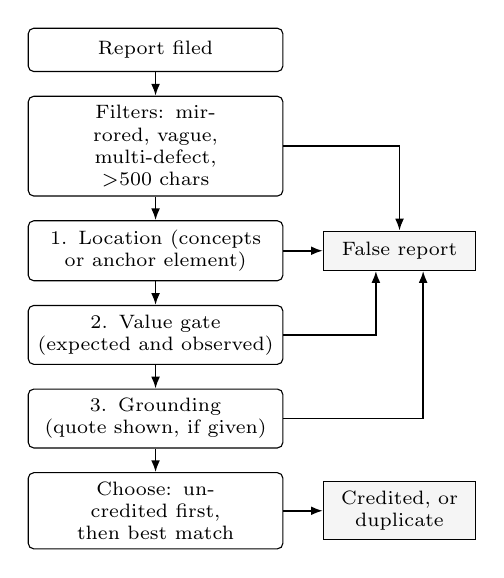
\begin{tikzpicture}[
      st/.style={draw, rounded corners=2pt, align=center, font=\scriptsize, text width=3.0cm, minimum height=5.5mm, fill=white},
      res/.style={draw, align=center, font=\scriptsize, text width=1.7cm, minimum height=5mm, fill=black!4},
      arr/.style={-{Latex[length=1.5mm]}, semithick}]
    \node[st] (r) {Report filed};
    \node[st, below=3mm of r] (f) {Filters: mirrored, vague,\\multi-defect, $>$500 chars};
    \node[st, below=3mm of f] (l) {1. Location (concepts\\or anchor element)};
    \node[st, below=3mm of l] (v) {2. Value gate\\(expected and observed)};
    \node[st, below=3mm of v] (g) {3. Grounding\\(quote shown, if given)};
    \node[st, below=3mm of g] (c) {Choose: uncredited first,\\then best match};
    \node[res, right=5mm of l] (fr) {False report};
    \node[res, right=5mm of c] (cr) {Credited, or\\duplicate};
    \foreach \a/\b in {r/f, f/l, l/v, v/g, g/c} \draw[arr] (\a) -- (\b);
    \draw[arr] (c) -- (cr);
    \draw[arr] (f.east) -| (fr.north);
    \draw[arr] (l) -- (fr);
    \draw[arr] (v.east) -| ([xshift=-3mm]fr.south);
    \draw[arr] (g.east) -| ([xshift=3mm]fr.south);
  \end{tikzpicture}
  \caption{Decision path of the deterministic matcher for one report.}
  \Description{A vertical flowchart: a report passes filters, location, value and grounding gates; a
  failure at any gate makes it a false report; a pass credits a matching regression.}
  \label{fig:grading}
\end{figure}

\paragraph{Validation.}
Table~\ref{tab:validation} summarises two validation corpora of 606 reports each, written without
access to the keys by agents that were shown the buggy and fixed behaviour. The matcher credits
84.2\% of correct reports and 9.9\% of near-miss or vague reports, and it never credits a report to
the wrong regression within its episode. The screen-grounded corpus exposes the matcher's main known
failure: a report that points at the right element but claims the wrong problem is credited in 35 of
101 cases. In addition, every report rejected in the Sonnet and Haiku runs (167) was judged by hand
against the transcripts: 113 described real app behaviour that is not a planted regression, 21 were
agent errors, 17 described a different symptom on the right feature, 4 duplicated a credited
regression, and 12 (8 distinct findings) described a planted regression that the matcher missed. The
keys of those regressions were widened before the remaining configurations were run, and the Sonnet
and Haiku runs were re-scored with the widened keys (Section~\ref{sec:threats}).

\begin{table}[t]
  \caption{Matcher validation on two corpora of 606 reports each.}
  \label{tab:validation}
  \small
  \begin{tabular}{@{}lr@{}}
    \toprule
    Corpus and report kind & Credited \\
    \midrule
    \multicolumn{2}{@{}l}{\emph{Blind corpus (404 correct, 202 near-miss or vague)}} \\
    \quad Correct reports & 84.2\% \\
    \quad Near-miss or vague reports & 9.9\% \\
    \quad Wrong regression within the episode & 0\% \\
    \midrule
    \multicolumn{2}{@{}l}{\emph{Screen-grounded corpus (101 per kind)}} \\
    \quad Careful, right element and quote & 94/101 \\
    \quad Right element, sloppy prose & 68/101 \\
    \quad Neighbouring element & 88/101 \\
    \quad Near-miss on another element & 5/101 \\
    \quad Same element, wrong problem & 35/101 \\
    \quad Vague, with a real quote & 0/101 \\
    \bottomrule
  \end{tabular}
\end{table}

\subsection{Metrics}
For episode $e$, let $B_e$ be its observable regressions, $C_e \subseteq B_e$ the credited ones, $F_e$
the number of false reports, $s_e \in \{0,1\}$ whether the agent signed off, and $k_e \in \{0,1\}$
whether the controller ended the session at the action cap or the report limit:
\begin{gather*}
\text{Recall} = \frac{\sum_e |C_e|}{\sum_e |B_e|},\qquad
\text{Strict pass} = \frac{1}{N}\sum_e \mathbf{1}\big[C_e = B_e \wedge s_e\big],\\
\text{Episode Score} = \frac{1}{N}\sum_e \mathrm{cc}(|C_e|,|B_e|)\cdot \pi_e \cdot \big(\tfrac{1}{2}\big)^{k_e},
\end{gather*}
where $\mathrm{cc}(c,b) = \frac{1+(c-1)/2}{1+(b-1)/2}$ for $c \ge 1$ and $\mathrm{cc}(0,b)=0$ is the
catch credit, and $\pi_e = |C_e|/(|C_e|+F_e)$ is the episode's report precision ($\pi_e = 1$ when
$|C_e|+F_e = 0$, a case that arises only with zero credit). Recall asks whether the agent finds the
regressions. Strict pass is the release-gate view: anything less either ships a regression or ends
without a verdict. The Episode Score values useful work that can be trusted: the first catch earns the
most, false reports discount it, and a session the controller had to end keeps half its credit. We
also report pooled report precision $\sum|C_e|/\sum(|C_e|+F_e)$, how each episode ended, and the cost
at API list prices.

\paragraph{Changelog coverage.}
For each release-note line we measure from the transcript, with no model involved, whether the agent
\emph{reached} the feature (one of its exact UI strings appeared in an observation), \emph{exercised}
it (six or more actions with the feature on screen), and \emph{caught} its regression. A miss is
\emph{ignored} (never reached), \emph{shallow} (reached, not exercised) or \emph{not noticed}
(exercised, not caught).

\paragraph{Statistics.}
The episode is the sampled unit, and regressions in one episode share a session.
\begin{itemize}[leftmargin=*]
\item \emph{Intervals.} Recall, precision and the Episode Score have 95\% percentile bootstrap
  intervals that resample whole episodes (2,000 resamples)~\cite{efron1979,field2007clustered}. Strict
  pass has Wilson intervals~\cite{wilson1927,brown2001interval}.
\item \emph{Pairwise tests.} For each metric, the 15 pairs of configurations are compared with a paired
  sign-flip permutation test over the 51 per-episode differences (20,000 permutations), and Holm's
  procedure corrects within each metric~\cite{holm1979}.
\item \emph{Other tests.} Catch overlap is compared with independence by a hypergeometric tail, Holm
  corrected over the 15 pairs, and summarised by the Jaccard index~\cite{jaccard1912}. Exact McNemar
  tests on discordant regressions~\cite{mcnemar1947}, Fisher's exact test for the fix-date
  split~\cite{fisher1922} and Spearman's $\rho$ across configurations~\cite{spearman1904} are
  reported uncorrected and treated as descriptive.
\item \emph{Confidence.} The area under the receiver operating characteristic curve (AUROC) is the
  probability that a correct sign-off states a higher confidence than an incorrect
  one~\cite{hanley1982auc}.
\end{itemize}
With 51 episodes, central-limit approximations can understate uncertainty~\cite{bowyer2025clt}, so
all tests use exact or resampling methods~\cite{miller2024errorbars}.

%% ------------------------------------------------------------------------------------------
\section{Experimental Setup}
\label{sec:setup}

\paragraph{Research questions.}
\rqref{1} How well can LLM agents hold a release gate (recall, strict pass, Episode Score)?
\rqref{2} Can their reports and sign-offs be trusted (precision, endings, confidence)?
\rqref{3} How do effort and cost relate to the score?
\rqref{4} Where and why do agents miss regressions?

\paragraph{Configurations.}
We evaluate each model in its vendor's own agent harness at the reasoning effort the harness uses by
default, and GPT-6 Luna also at maximum effort (Table~\ref{tab:configs}). Each harness runs headless
with its built-in tools disabled and only the device server attached. No configuration is given more
actions, time or reports than another. Each configuration ran all 51 episodes once, three containers
in parallel. We refer to configurations by the short names in Table~\ref{tab:configs}. Two
episode-prompt versions were used; they differ only in the sign-off instruction
(Appendix~\ref{app:prompt} and Section~\ref{sec:threats}).

\begin{table}[t]
  \caption{Agent configurations. AA: Artificial Analysis Intelligence Index v5.0.1~\cite{aa2026index}
  for the same model and effort (``--'': no matching entry). Def.: the harness default. Prompt:
  episode-prompt version.}
  \label{tab:configs}
  \footnotesize\setlength{\tabcolsep}{2.4pt}
  \begin{tabular}{@{}llllcr@{}}
    \toprule
    Short name & Model & Harness & Effort & Prompt & AA \\
    \midrule
    Sonnet & Claude Sonnet 5.5 & Claude Code & medium (def.) & v4 & 31 \\
    Haiku & Claude Haiku 5.5 & Claude Code & def. & v4 & -- \\
    Sol & GPT-6.1 Sol & Codex CLI & low (def.) & v4.1 & 35 \\
    Luna med. & GPT-6 Luna & Codex CLI & medium (def.) & v4.1 & 18 \\
    Luna max & GPT-6 Luna & Codex CLI & max & v4.1 & 28 \\
    DeepSeek & DeepSeek V4.1 Flash & DeepSeek Harness & high & v4 & -- \\
    \bottomrule
  \end{tabular}
\end{table}

%% ------------------------------------------------------------------------------------------
\section{Results}
\label{sec:results}

\begin{table*}[t]
  \caption{Main results on 51 episodes (one run per configuration). Recall and Episode Score: 95\%
  bootstrap CI over episodes; strict pass: Wilson 95\% CI. Cost: mean cost per episode at API list
  prices; $^\ast$one session has no token record, so the mean is over 50.}
  \label{tab:main}
  \small
  \begin{tabular}{@{}lrrrrrr@{}}
    \toprule
    Configuration & Recall (\%) & Strict pass (\%) & Precision (\%) & Episode Score & Actions & \$/episode \\
    \midrule
    Sol & \textbf{59.3} [50.0, 68.5] & \textbf{29.4} [18.7, 43.0] & 34.0 & 0.29 [0.22, 0.36] & 202 & 0.65 \\
    DeepSeek & 50.5 [40.0, 60.4] & 11.8 [5.5, 23.4] & 34.1 & 0.18 [0.12, 0.25] & 294 & 0.06 \\
    Sonnet & 46.2 [36.3, 55.7] & 23.5 [14.0, 36.8] & 44.2 & \textbf{0.39} [0.29, 0.50] & 67 & 0.54 \\
    Haiku & 42.9 [31.1, 53.9] & 13.7 [6.8, 25.7] & 27.7 & 0.24 [0.16, 0.32] & 217 & 0.64 \\
    Luna max & 34.1 [23.9, 44.0] & 11.8 [5.5, 23.4] & 24.4 & 0.21 [0.13, 0.29] & 166 & 0.16$^\ast$ \\
    Luna med. & 15.4 [8.6, 23.2] & 3.9 [1.1, 13.2] & \textbf{50.0} & 0.14 [0.07, 0.22] & 39 & 0.02 \\
    \bottomrule
  \end{tabular}
\end{table*}

\begin{figure*}[t]
  \centering
  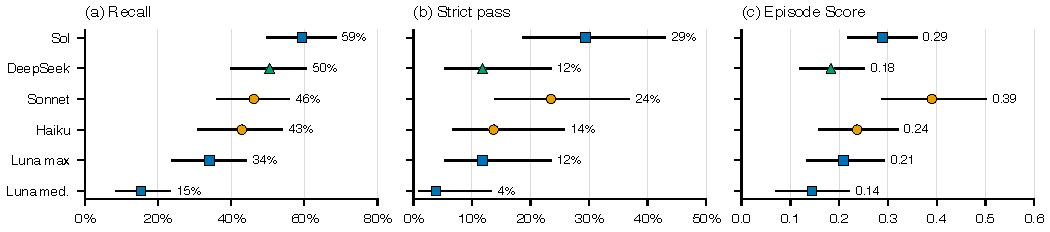
\includegraphics[width=\textwidth]{figs/headline.pdf}
  \caption{Headline metrics with 95\% intervals (Table~\ref{tab:main}). Colour and marker shape encode
  the provider. Rows are ordered by recall.}
  \Description{Three dot-and-interval panels for recall, strict pass and Episode Score across six
  agent configurations.}
  \label{fig:headline}
\end{figure*}

\subsection{RQ1: Holding the Gate}
Table~\ref{tab:main} and Figure~\ref{fig:headline} give the main results. The best recall is 59.3\%
(Sol) and the best strict pass rate is 29.4\%: in about seven of ten releases even the best
configuration ships a regression or ends without a verdict. Over all six configurations, 74 of the 91
observable regressions (81\%) are caught at least once and 17 are caught by none.

After Holm correction, Sol and DeepSeek have higher recall than Luna max, and Sol, DeepSeek, Sonnet
and Haiku have higher recall than Luna med.\ ($p_{\text{Holm}} \le 0.011$). No difference among Sol,
DeepSeek, Sonnet and Haiku is significant. Sol catches 22 regressions that Sonnet misses and Sonnet
catches 10 that Sol misses; the mean per-episode recall difference is $+0.15$ ($p_{\text{Holm}} =
0.17$; exact McNemar $p = 0.050$, uncorrected). On strict pass, only Sol against Luna med.\ is
significant ($p_{\text{Holm}} = 0.015$).

\answer{1}{No configuration holds the gate reliably. The best catches 59\% of the regressions and
passes 29\% of the releases strictly, and the four strongest configurations do not differ
significantly in recall.}

\subsection{RQ2: Trusting Reports and Sign-Offs}

\begin{figure}[t]
  \centering
  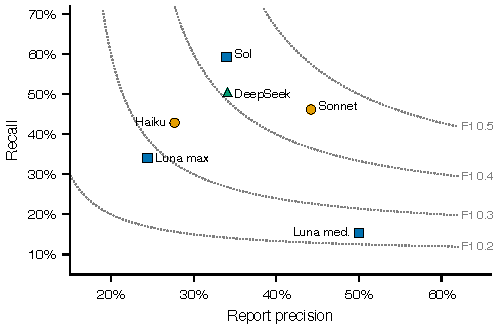
\includegraphics[width=\columnwidth]{figs/recall_precision.pdf}
  \caption{Recall against report precision. Dotted lines join points of equal F1.}
  \Description{Scatter plot of six configurations by report precision and recall with iso-F1 curves.}
  \label{fig:rp}
\end{figure}

\paragraph{Finding versus trusting.}
The configuration that finds the most regressions is not the one with the most trustworthy output
(Figure~\ref{fig:rp}). Sol files 164 reports, of which 54 are credited (precision 34\%); Sonnet files
99, of which 42 are credited (44\%). With precision counted, Sonnet has the highest Episode Score
(0.39). Its lead is significant over DeepSeek, Luna max and Luna med.\ ($p_{\text{Holm}} \le 0.006$),
but not over Haiku ($p_{\text{Holm}} = 0.058$) or Sol ($+0.10$, $p_{\text{Holm}} = 0.66$). At this
sample size, Sol's first place on recall and Sonnet's first place on the Episode Score are both
descriptive.

\begin{figure}[t]
  \centering
  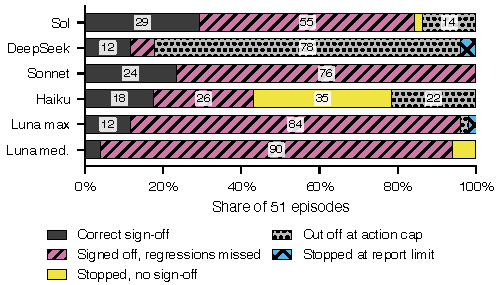
\includegraphics[width=\columnwidth]{figs/endings.pdf}
  \caption{How each of the 51 episodes ended. Hatching repeats the colour coding.}
  \Description{Stacked horizontal bars of episode endings per configuration.}
  \label{fig:endings}
\end{figure}

\paragraph{Stopping.}
Figure~\ref{fig:endings} shows how episodes ended. Sonnet and both Luna settings sign off in almost
every episode, but 76--90\% of all their episodes end in a sign-off with regressions still present.
DeepSeek is cut off at the action cap in 78\% of episodes. Haiku stops without signing off in 35\%,
mostly because, under prompt v4, it would not sign off while reported bugs remained
(Section~\ref{sec:threats}). No configuration signs off correctly in more than 29\% of episodes.

\begin{figure}[t]
  \centering
  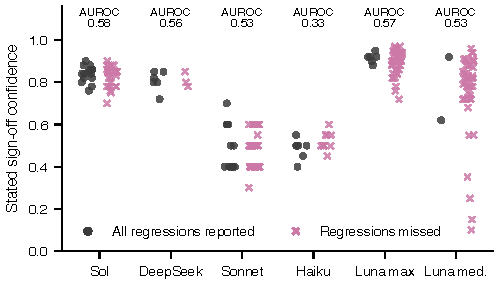
\includegraphics[width=\columnwidth]{figs/confidence.pdf}
  \caption{Stated sign-off confidence for sign-offs after which every regression had been reported
  (circles) and sign-offs that left regressions (crosses), with the AUROC per configuration.}
  \Description{Strip plot of sign-off confidence by configuration, split by whether the sign-off was correct.}
  \label{fig:conf}
\end{figure}

\paragraph{Confidence.}
The confidence an agent states with its sign-off does not separate correct from incorrect sign-offs
(Figure~\ref{fig:conf}): the AUROC lies between 0.53 and 0.58 for five configurations and is 0.33 for
Haiku, whose confidence is slightly inverted. Each configuration instead has a typical value: about
0.5 for Sonnet and Haiku and 0.75--0.9 for the GPT and DeepSeek configurations. Self-reported
confidence of language models can be calibrated in some formats~\cite{kadavath2022know}, and neural
networks are often miscalibrated~\cite{guo2017calibration}. In \aqb the stated confidence carries no
usable signal for a release decision.

\answer{2}{Not yet. The configuration with the highest recall files two false reports for each
credited one, most sign-offs leave regressions in the build, and stated confidence is close to chance
at telling a safe sign-off from an unsafe one.}

\subsection{RQ3: Effort and Cost}

\begin{figure*}[t]
  \centering
  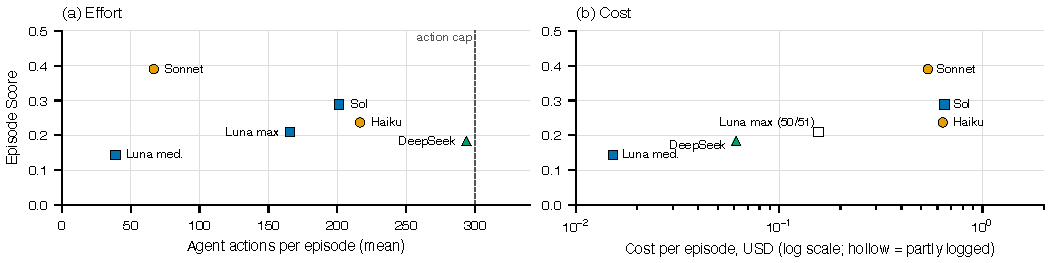
\includegraphics[width=\textwidth]{figs/effort_cost.pdf}
  \caption{Episode Score against (a) mean agent actions per episode (dashed: the 300-action cap) and
  (b) cost per episode at API list prices (log scale). Hollow marker: cost known for 50 of 51 sessions.}
  \Description{Two scatter plots of Episode Score against actions and against cost.}
  \label{fig:effort}
\end{figure*}

Across configurations, the number of actions does not predict the Episode Score (Spearman
$\rho = 0.03$, $n=6$; Figure~\ref{fig:effort}a). Sonnet scores highest with 67 actions per episode;
Sol, Haiku and DeepSeek use 200--300 and score lower. Within one model, more effort does help: raising
GPT-6 Luna from medium to maximum effort raises its actions from 39 to 166 per episode, the changed
features it exercises from 27 to 66 of 92, recall from 15\% to 34\% and the Episode Score from 0.14
to 0.21, while precision falls from 50\% to 24\%. Cost and Episode Score are positively associated
across configurations ($\rho = 0.83$, $n=6$; Figure~\ref{fig:effort}b). With six points this is
descriptive.

For the four configurations with a matching Artificial Analysis entry~\cite{aa2026index}, the index
and the Episode Score rank them similarly ($\rho = 0.80$, $n=4$). The one reversal is Sol (index 35)
and Sonnet (index 31), which \aqb orders the other way.

\answer{3}{Across configurations, more actions do not mean a higher score, and cost is weakly
informative at best. Within GPT-6 Luna, more reasoning effort raised recall and the score.}

%% ------------------------------------------------------------------------------------------
\section{RQ4: Where Agents Miss}
\label{sec:rq4}

\begin{figure}[t]
  \centering
  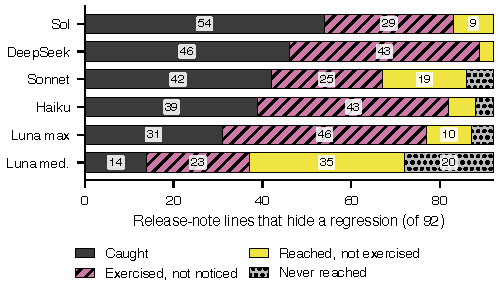
\includegraphics[width=\columnwidth]{figs/coverage.pdf}
  \caption{What happened to each of the 92 release-note lines that hide a regression.}
  \Description{Stacked bars partitioning 92 lines into caught, exercised but not noticed, reached but
  not exercised, and never reached.}
  \label{fig:coverage}
\end{figure}

\paragraph{Agents reach the changed features but do not expose their regressions.}
Every configuration except Luna med.\ reaches 78--88 of the 92 changed features, and Sol and DeepSeek
reach all but four and five of them (Figure~\ref{fig:coverage}). The misses lie in what agents do
there: 23--46 regressions per configuration sit in features the agent exercised with six or more
actions without exposing them. Sonnet looks at features briefly: 23 of its 42 catches came from
features it looked at for fewer than six actions, more than any other configuration (10--15), and it
also has the most shallow misses among the strong configurations (19).

\begin{figure*}[t]
  \centering
  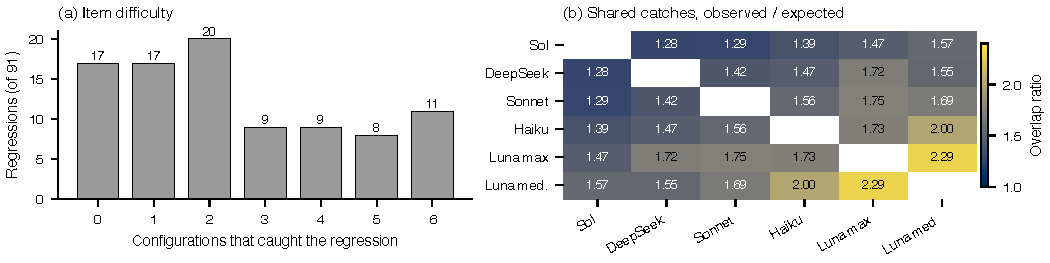
\includegraphics[width=\textwidth]{figs/difficulty.pdf}
  \caption{(a) Number of configurations that caught each observable regression. (b) For each pair of
  configurations, shared catches divided by the number expected if they caught regressions
  independently; every ratio exceeds 1 ($p_{\text{Holm}} \le 0.022$, hypergeometric tail).}
  \Description{Histogram of catches per regression and a heat map of pairwise overlap ratios.}
  \label{fig:difficulty}
\end{figure*}

\paragraph{Configurations share a difficulty structure.}
Catches overlap more than chance for all 15 pairs of configurations (Figure~\ref{fig:difficulty}b):
the ratio of observed to expected shared catches is 1.28--2.29, and the Jaccard index 0.22--0.54. For
Sol and Sonnet, 32 shared catches compare with 24.9 expected under independence. The number of
configurations that catch a regression covers the whole range (Figure~\ref{fig:difficulty}a): 17
regressions are caught by none and 11 by all six. This pattern suggests stable per-regression
difficulty, which an item-response model could estimate directly~\cite{chen2025irt}.

\begin{table}[t]
  \caption{Recall (\%) by app group, upstream fix date and regression family.}
  \label{tab:splits}
  \footnotesize\setlength{\tabcolsep}{2.6pt}
  \begin{tabular}{@{}lrrrrrrr@{}}
    \toprule
    Split & $n$ & Sol & DeepSeek & Sonnet & Haiku & Luna max & Luna med. \\
    \midrule
    Mature apps & 51 & 56.9 & 51.0 & 49.0 & 41.2 & 41.2 & 5.9 \\
    2026 apps & 40 & 62.5 & 50.0 & 42.5 & 45.0 & 25.0 & 27.5 \\
    \midrule
    Fixed before 2026 & 33 & 57.6 & 48.5 & 51.5 & 42.4 & 42.4 & 9.1 \\
    Fixed in 2026 & 58 & 60.3 & 51.7 & 43.1 & 43.1 & 29.3 & 19.0 \\
    \midrule
    State & 37 & 56.8 & 51.4 & 45.9 & 37.8 & 35.1 & 8.1 \\
    Display & 35 & 62.9 & 54.3 & 51.4 & 48.6 & 34.3 & 25.7 \\
    Interaction & 19 & 57.9 & 42.1 & 36.8 & 42.1 & 31.6 & 10.5 \\
    \bottomrule
  \end{tabular}
\end{table}

\paragraph{Splits.}
Table~\ref{tab:splits} breaks recall down. No split changes the ordering of the four strongest
configurations by more than one place, and Luna med.\ does far worse on the mature apps (5.9\%) than
on the 2026 apps (27.5\%).

\paragraph{The regressions both leading configurations miss.}
The 27 regressions that both Sol and Sonnet missed are not older or newer than the rest, and were not
ported with lower confidence. They fall into four groups by what a tester must do to expose them.
\begin{itemize}[leftmargin=*]
\item Round trip (6): change a setting, close and reopen the file or app, and check the value; for
  example an editor's indent size or the deck chosen for new notes.
\item Specific input or action (10): for example, long-pressing \emph{Bold} (which closes the app),
  choosing \emph{Select all} twice, typing seven digits into a five-digit field, or renaming
  ``French'' to ``FRENCH''. Sol and DeepSeek spent 133 and 151 actions on the Markor formatting
  toolbar without long-pressing \emph{Bold}.
\item Knowing the correct value (10): the screen looks plausible, as with 2,567,890 coins shown as
  2.6M where the format floors to 2.5M, a Videos filter that says ``No photos found'', or ``04:00''
  among times written in AM/PM (Figure~\ref{fig:hard}).
\item Multi-step state (1): a favourite star that goes out of sync after a dialog.
\end{itemize}
The first two groups correspond directly to instructions in the prompt (``after a change, leave and
come back, and check that it was kept''; ``try empty, boundary and unusual values''), and the prompt
states that signing off with bugs unreported is the worst outcome. In the episodes where Sonnet missed
a regression it signed off after about 70 actions on average. The logged actions show how rarely the
method's checks were run: Sonnet re-opened the app in 13 of 51 episodes and rotated the device in 23,
and Sol rotated the device in every episode but long-pressed an element in only 7.

\begin{figure*}[t]
  \centering
  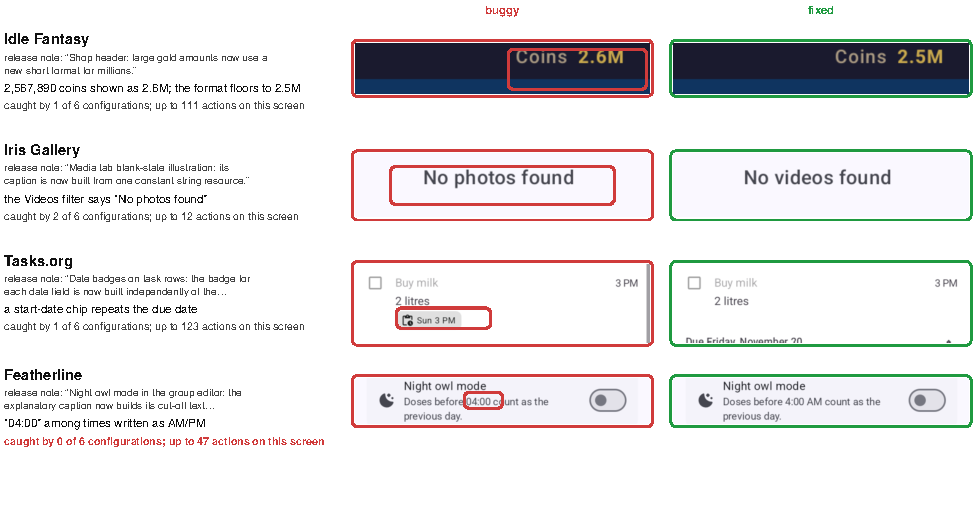
\includegraphics[width=0.8\textwidth]{../figures/p7_hard.pdf}
  \caption{Regressions that both Sol and Sonnet missed, as the device shows them on the buggy and fixed
  builds (calibration screenshots; the defect circled), with the release-note line the agent received.}
  \Description{Four rows of paired buggy and fixed screenshots with release-note text.}
  \label{fig:hard}
\end{figure*}

\paragraph{Contamination.}
If agents had memorised the upstream fixes, older regressions would be easier. Comparing regressions
fixed before 2026 (33) with those fixed in 2026 (58), no configuration differs significantly (Fisher's
exact test, all $p \ge 0.24$; differences from $-13$ to $+10$ percentage points with no consistent
sign). We find no evidence of a date effect. This tests the fix date, not each model's training
cut-off, so it cannot rule out contamination~\cite{sainz2023contamination}.

\answer{4}{Agents miss regressions in features they did exercise, because they skip the specific
check that exposes them: a round trip, a particular input, or a comparison with the correct value.
Hard regressions are hard for every configuration.}

%% ------------------------------------------------------------------------------------------
\section{Discussion}

\paragraph{Which metric for which gate.}
If a person reviews the agent's reports before release, a missed regression is the costly error and
recall ranks the configurations; there Sol leads, although not significantly against DeepSeek, Sonnet
or Haiku. If reports go to developers directly, precision and correct sign-off matter and the Episode
Score ranks the configurations; there Sonnet leads, again not significantly against Sol. For an
unattended gate, strict pass is the relevant metric.

\paragraph{What may help.}
The misses concentrate in verification steps the agents were told to use. Scaffolding that enforces
the method, for example a checklist of round trips and boundary inputs for each changed feature, may
therefore help more than a larger exploration budget. Because stated confidence is uninformative, a
gate should not use it to decide whether to ship.

\paragraph{Headroom.}
The union of all six configurations still misses 19\% of the regressions. Because real but unplanted
behaviour counts as a false report, the Episode Score of a perfect agent can fall slightly below 1;
recall and strict pass have no such ceiling.

\paragraph{Limitations and future work.}
\aqb plants real regressions into a pinned head rather than observing regressions as they arise in
development, and it covers 9 apps on one emulated device. It has no human-tester baseline and no
non-LLM baseline such as an automated GUI test generator. Each configuration ran once. Future work
should add a human baseline on a subset of episodes, repeated runs, more apps and devices, and a
second, independently written set of release notes.

%% ------------------------------------------------------------------------------------------
\section{Threats to Validity}
\label{sec:threats}
We follow the standard classification of validity threats~\cite{wohlin2012experimentation}.

\paragraph{Internal validity.}
(i) \emph{Prompt version.} Sonnet, Haiku and DeepSeek ran episode prompt v4, which asked agents to sign
off when the areas had ``no remaining bugs''. Under the fast protocol a reported bug stays in the
build, so an agent that had reported a bug could not sign off truthfully. Sol and both Luna settings
ran v4.1, which asks agents to sign off once they have tested the areas and reported every bug they
found (Appendix~\ref{app:prompt}). Endings that withhold sign-off only for this reason are counted as
sign-offs in Figure~\ref{fig:endings}, but strict pass requires an actual sign-off, so every sign-off
metric (strict pass, endings, confidence) is confounded with the prompt version. Recall and precision
do not depend on this rule. (ii) \emph{Harness and model.} Each model ran in its vendor's harness at
its default effort, so harness and model effects are not separated. (iii) \emph{Grader development.}
Match keys for 8 regressions were widened after a manual review of the rejected reports of the Sonnet
and Haiku runs, which were then re-scored. This added 5 credited regressions for Sonnet and a net 2
for Haiku: before widening, Sonnet's recall was 40.7\% and its strict pass 17.6\%, and Haiku's recall
was 40.7\% with an unchanged strict pass. The other configurations were graded live with the widened
keys, and their rejected reports were not reviewed by hand, so a matcher miss specific to them would
not have been corrected. (iv) \emph{Single run.} Each configuration ran each episode once. Repeated
runs reduce prediction noise substantially~\cite{wang2025noises}, and part of the difference in which
regressions each configuration caught is run-to-run variance.

\paragraph{Construct validity.}
(i) The matcher credits 84\% of correct reports in its blind validation, so recall is a lower bound
relative to reports a person would accept. (ii) It credits 35 of 101 validation reports that name the
right element but the wrong problem, which can inflate recall. (iii) 21 of the 226 credited
regressions across all runs rest on reports without a checked quote; requiring a quote for every
report would lower recall by 0--7 points per configuration and would put Haiku (42.9\%) above Sonnet
(40.7\%). (iv) Release notes were written by the authors in changelog style, and some lines are more
specific than others. (v) Costs come from each harness's own cost line; for 28 DeepSeek sessions
stopped at the action cap they are summed from per-step token usage at DeepSeek list prices. (vi) The
two validation corpora were written by agents, not people.

\paragraph{External validity.}
\aqb has 9 apps, 51 episodes and 92 regressions, on one emulated device configuration. Five apps have
a history only from 2026. Device checks ran once per build, and two regressions depend on environment
details (the order of equal sort keys and the device's 12-hour clock). Maximum effort was evaluated
only for GPT-6 Luna, and the largest model of each provider was not evaluated.

\paragraph{Conclusion validity.}
With six configurations and 51 episodes, most pairwise differences among the stronger configurations
are not significant after correction. The exact McNemar tests treat regressions as independent
although they are grouped in episodes, so the main tests permute whole episodes. Recall intervals that
resample episodes are 0.91--1.13 times as wide as Wilson intervals over regressions, so the grouping
is weak. All correlations across configurations have $n \le 6$ and are descriptive.

%% ------------------------------------------------------------------------------------------
\section{Ethics and Broader Impact}
All apps are open source and used under their licences (GPL-3.0 or Apache-2.0); modified builds are
distributed only with source, as the GPL requires. No human participants or personal data were
involved; agent transcripts contain only seeded test data. The answer material is withheld from the
public release so that the benchmark cannot be trained on directly. Our results argue against
replacing a human release gate with an LLM agent at the current level of performance; a deployment
that did so would ship regressions in most releases.
% AUTHOR TODO: add the venue's required statement on the use of generative AI tools, if any.

%% ------------------------------------------------------------------------------------------
\section{Data Availability}
The dataset (apps, bugs, checks, episodes and briefs), the device server, the controller, the matcher,
all six stored runs with full transcripts, and the scripts that regenerate every number, table and
figure in this paper are provided as an open artifact at \url{https://github.com/mynk8/android-qa-bench}. The answer material (original
fixes, forward-port patches and the release-note key) is kept out of the public release, and a script
exports and checks the public tree. Unit tests, a leak scan, a replay check that reproduces every
stored grading decision with the current keys, and a byte-identical regeneration of the paper data run
in continuous integration~\cite{collberg2016repeatability}.

%% ------------------------------------------------------------------------------------------
\section{Conclusion}
Current LLM agents reach most of the features a release changed, but they do not yet hold a release
gate: they skip the specific checks that expose regressions, and the confidence they state when they
sign off cannot be used to decide whether to ship. \aqb makes these failures measurable with
device-verified regressions and deterministic grading, and its hardest regressions, the 17 that no
configuration caught, give a concrete target for the next generation of testing agents.

\bibliographystyle{ACM-Reference-Format}
\bibliography{refs}

\appendix

\section{Prompt Text}
\label{app:prompt}
The QA method given to every agent:
\begin{lstlisting}
How to test well (general QA practice):
- Make a plan from the areas above and exercise every one of them before you sign off.
  Signing off while bugs remain unreported is the worst outcome, worse than spending
  more steps.
- Go past the happy path. For each feature, also check:
  - State: after a change, leave and come back, and check that it was kept.
  - Reversal: undo, cancel or reverse a change, and check the app returns to the
    right state.
  - Repetition: repeat an action, and check the result is still right.
  - Input: try empty, boundary and unusual values.
  - Consistency: check that what each screen shows agrees with the data, and with
    other screens.
  - Device: rotate the screen, and check that nothing is lost.
  - Navigation: reach screens by more than one route.
- Use the starting data described in the preconditions in your tests.
- Reproduce a problem once before you report it.
\end{lstlisting}
The only difference between prompt versions is the sign-off instruction. Version v4:
\begin{lstlisting}
- When you believe the areas have no remaining bugs, call `sign_off`.
  The session then ends.
\end{lstlisting}
Version v4.1:
\begin{lstlisting}
- When you have tested the areas and filed a report for every bug you found, call
  `sign_off`. Bugs you have already reported do not stop you from signing off.
  The session then ends.
\end{lstlisting}

\section{Example Match Key}
\label{app:key}
The key for the Iris Gallery regression in which the Videos filter shows ``No photos found''
(Figure~\ref{fig:hard}). Each inner list is one concept group; a trailing \texttt{*} matches a word
prefix.
\begin{lstlisting}
screens:           media tab, media, main, gallery
elements:          empty message, empty state      fields: message
location_concepts: empty*, message, placeholder, blank*, wording, text
symptom_types:     wrong_value
expected_concepts: [no videos, videos found, video*, movie*, film*, placeholder,
                    wrong kind, media type]
observed_concepts: [no photos, photos found, photo*, mentions photos, picture*,
                    image*, wording]
\end{lstlisting}

\end{document}
